\newpage
\subsection{Building of TSEngine}
\label{sec:build}
\hspace{\parindent} The main purpose of creating a sophisticated building system is to assure the project is multiplatform, non-device dependent and is easy to set up.\\ This is necessary for long-living and non-single developer projects.
To fulfill those guidelines, the core of every modern C++ project is \hyperref[sec:stack_cmake]{CMake}, and this is no different in our project.
A comprehensive series of articles about types of libraries in C++ from Medium \textit{"Cpp Libraries"} \cite{cpplibs} can be a great source of knowledge that is useful in this section.
Our building is based on \hyperref[sec:stack_cmake]{\ref*{sec:stack_cmake} CMake} that recently has become the leading tool in building C++ systems; \hyperref[sec:cmake]{\ref*{sec:cmake} TSEngine's CMake}.
\subsubsection{Build Structure}
\hspace{\parindent} Followed figure shows the build structure of TSEngine:
\label{fig:build_struct}
\begin{figure}[h]
  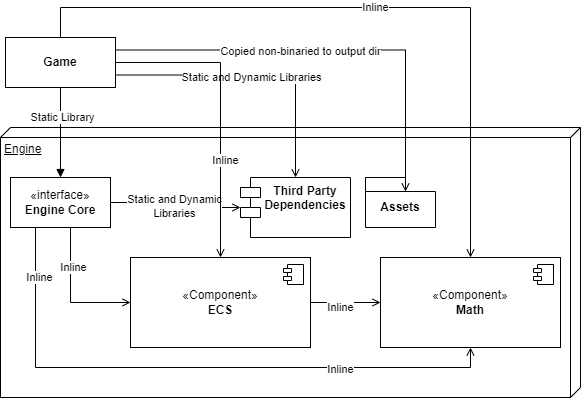
\includegraphics[width=\linewidth]{figures/build.png}
  \caption{Build Structure}
\end{figure}
Currently, TSEngine is delivered to the game in the form of static library, unfortunately at the moment of writing this thesis we haven't yet implemented dynamic version of TSEngine, but we provided abstraction and architecture to do it.
As the \ref{fig:build_struct} presents, engine is consisted of two other components: Entity Component System(ECS) and Math libraries which are header only template libraries where it is possible in compile time, both can be optionally included.

Besides of it, as was said in the previous paragraph as far now the engine can be built only as static library all third party dependencies must be added to the executable.\\
Assets are copied to the output directory whenever the engine or game is built. This fragment deservers further attention, because it creates a problem while compiling shaders - what mentioned is in \hyperref[problem_with_shader_compilation]{Shader Compiler} section. However, would be also nice to store assets in binary packages for the game usage, what is common practice nowadays, with an addition of serialization of game's structures and storing it, it would create a pretty functional system.

\begin{verbatim}
├───engine
│   ├───CMakeLists.txt
│   └───tests
│       └───CMakeLists.txt
├───external
│   └───CMakeLists.txt
├───game
│   └───CMakeLists.txt
└───CMakeLists.txt
\end{verbatim}
\begin{table}[h]
\caption{CMake files}
\end{table}
\newpage
\subsubsection{Instruction How To Build the Project}
\hspace{\parindent} Instructions which are needed to build the project:
\label{sec:how_to_run}
\begin{enumerate}
    \item Be sure that you have already installed and updated graphics drivers and your GPU's capabilities are enough- \hyperref[sec:hardware]{supported hardware}
    \item Be sure that you have already installed all needed VR headset software and set up the environment to play - \hyperref[sec:hardware]{supported hardware}
    \begin{enumerate}
        \item Optional Virtualizer: If you want to use \hyperref[sec:virtualizer]{Virtualizer}, be sure to have all needed software installed and set up the treadmill to play.
    \end{enumerate}
    \item Download Git if you don't have yet:
        \href{https://git-scm.com/downloads}{https://git-scm.com/downloads}
    \item Download CMake if you don't have yet:
        \href{https://cmake.org/download/}{https://cmake.org/download/}
    \item Download Visual Studio with C++ workspace if you don't have yet:
        \href{https://visualstudio.microsoft.com/vs/}{https://visualstudio.microsoft.com/vs/}
    \item Open system terminal
    \item Run command (cloning the repository):\\
        \texttt{git clone https://github.com/damian-tomczak/tsengine --recursive \&\& cd tsengine}
    \begin{enumerate}
        \item Optional Virtualizer: If you want to use \hyperref[sec:virtualizer]{Virtualizer}, move Cyberith SDK to \texttt{external/CybSDK\_Cpp} or set \texttt{CYBSDK\_DIR} with the path to where the SDK is unpacked during TSEngine configuration (\ref{proj_conf})
    \end{enumerate}
    \item Run command (creating working directory):\\
        \texttt{mkdir build \&\& cd build}
    \item Run command (creating project files - on Windows by default Visual Studio project if is installed, othwerwise use \texttt{-G} flag):\\
        \texttt{cmake ..}
    \label{proj_conf}
    \item Build the project with your build system.
    \item Run the project: \texttt{./build/output/tsgame/[BUILD TYPE]/tsgame.[EXECUTABLE FORMAT]}
\end{enumerate}

\subsubsection{Third Party Dependencies}
\label{sec:3rdparty}
\hspace{\parindent} We prioritize building from source code over using precompiled binaries.
One of the modern way of handling compiling from source code is to use git submodules. The core of this method is \texttt{.gitsubmodules} file containing all used external dependencies.
\begin{lstlisting}[caption=.gitsubmodules]
[submodule "external/vulkan"]
	path = external/vulkan
	url = https://github.com/KhronosGroup/Vulkan-Headers.git
[submodule "external/glslang"]
	path = external/glslang
	url = https://github.com/KhronosGroup/glslang
[submodule "external/googletest"]
	path = external/googletest
	url = https://github.com/google/googletest
[submodule "external/openxr"]
	path = external/openxr
	url = https://github.com/KhronosGroup/OpenXR-SDK.git
[submodule "external/tinyobjloader"]
	path = external/tinyobjloader
	url = https://github.com/tinyobjloader/tinyobjloader.git
\end{lstlisting}
The major advantage of source code dependencies over precompiled binaries is having significantly less memory usage to store a project and easy way to make a fork of your dependency. However, the biggest disadvantage of source code lies on compilation time.

\subsubsection{Cyberith SDK}
\label{sec:build_cybsdk}
\hspace{\parindent} There is one external dependency that git submodules doesn't cover, that dependency is Cybertith SDK, responsible for communication with Cyberith Virtualizer ELITE 2 treadmill - \hyperref[sec:virtualizer]{\ref*{sec:virtualizer} Virtualizer}.\\
This is the only 3rd party library that is included to the project as a binary and is optional to use.\\
To use treadmill, Cyberith SDK must be unpacked to the project, while its configuration - \hyperref[sec:how_to_run]{\ref*{sec:how_to_run} Instruction How To Buld the Project} section contains elaborated information about it.  

\subsubsection{Precompiled Header}
\hspace{\parindent} To reduce the amount of code which you care about adding in every translation unit, a precompiled header can be used. In our project we used it to reduce the amount of often used include directives, actually we used it only to don't mess up with adding STL for the engine's part.\\
More systemized and modern substitution of a precompiled header is C++20's Modules, simplicity-wise precompiled fragments of code. Unfortunately, when we started working on engineering thesis the implementation of it was still in bad condition, especially on the top of CMake. For the end of 2023 year, it is safe to use Modules with CMake for enthusiast projects, so no matter how you look at it, for an instance our engine.

\begin{lstlisting}[caption=Adding precompiled header(./engine/CMakeLists.txt)]
target_precompile_headers(${PROJECT_NAME} PUBLIC src/pch.h)
\end{lstlisting}

\subsubsection{Building Operating System Specific}
\label{sec:build_os}
\hspace{\parindent} Multiplatform building is covered by followed \texttt{os\_files}\ref{lst:os} function that removes from the \texttt{SRC\_FILES} variable all \texttt{*.cpp} files not designed to be used on platform that is currently used to build the project.
\label{lst:os}
\begin{lstlisting}[caption=os\_files function (./engine/CMakeLists.txt)]
function(os_files files_list_name regex)
    set(files_list ${${files_list_name}})
    list(FILTER files_list EXCLUDE REGEX "src/os/*")

    set(OS_FILES)
    if (WIN32)
        file(GLOB_RECURSE OS_FILES
            src/os/win32/${regex}
        )
    else()
        message(FATAL_ERROR "Not implemented")
    endif()

    list(LENGTH OS_FILES OS_FILES_LENGTH)
    if (OS_FILES_LENGTH EQUAL 0)
        message(FATAL_ERROR "Files specific for your system couldn't be found")
    endif()

    list(APPEND files_list ${OS_FILES})
    set(${files_list_name} ${files_list} PARENT_SCOPE)
endfunction()

file(GLOB_RECURSE SRC_FILES
    src/*.cpp
)

os_files(SRC_FILES *.cpp)
\end{lstlisting}

As we will discuss it in \hyperref[sec:problems]{\ref{sec:problems} Problems During the Development} section, we encountered problems with virtual reality on Linux systems, therefore to keep up the project open for further modifications and good practices we delivered layers of abstraction and where it was obvious errors are invoked with messages pointing that the followed code wasn't yet implemented for currently being built platform.\\ At the level of CMake, this problem handles \texttt{message} function with \texttt{FATAL\_ERROR} argument that stops the configuration of the project.\\ On the other hand, \texttt{\#error not implemented} preprocessor command secures this code at the level of C++.

\subsubsection{Common ABI}
\label{sec:build_abi}
\hspace{\parindent} When developing any library it is important to care about application binary interface (ABI), because the user of your product may not used the same headers used to build your library for plenty of reasons, especially when the library is dynamically linked, then a lot of opportunities for it appears.\\To avoid it you must oversee your ABI, we took it into the account but within the project's deadline was coming, exceptions from it had started to appear. One of those exceptions representant is Entity Component System's header file - \texttt{ecs.hpp} where there is no prepared any kind of intermediate interface between ECS's header and the engine.\\Therefore to provide just any kind of protection on the top of that we prepared \texttt{TS\_VER} preprocessor definition being a name of namespace - \hyperref[sec:namespaces]{\ref*{sec:namespaces} Namespaces}. But it is a partially solution because we must be aware that a change or addition to the engine breaks the exisiting ABI and update the version of the engine in the main CMake. 

\subsubsection{Preprocess Definitions}
\hspace{\parindent} Publicly exposed the engine's preprocessor definitions are: \texttt{ENGINE\_NAME} and \texttt{TS\_VER}.\\ First containing the \texttt{PROJECT\_NAME} variable so \texttt{tsengine} (so far it is used for creating Khronos's APIs' Instances because they take engine's name).\\ The latter assures \hyperref[sec:build_abi]{\ref{sec:build_abi} Common ABI}.
On the other hand private preprocessor definitions are: \texttt{VK\_USE\_PLATFORM\_\${VK\_USE\_PLATFORM}\_KHR} that is required by Vulkan headers to choose appropriate declaration based on system in use, \texttt{VK\_NO\_PROTOTYPES} is similar to the previous definition because is related to the Vulkan Headers dependency but this one turns off default Vulkan Loader this dependency comes with - \hyperref[sec:3rdparty]{\ref*{sec:3rdparty} Third Party Dependencies}, \texttt{XR\_USE\_GRAPHICS\_API\_VULKAN} is required for OpenXR to know which graphics API you use, \texttt{CYBSDK\_FOUND} this one is defined if Cyberith SDK is found - \hyperref[sec:build_cybsdk]{\ref*{sec:build_cybsdk} Cyberith SDK}, \texttt{TESTER\_ADAPTER} is defined when tests are enabled, which are by default enabled, \texttt{NOMINMAX} the purpose of it to disable \texttt{min}, \texttt{max} preprocessor functions defined in Windows API causing problems with STL.
\begin{lstlisting}[caption=Engine's preprocessor definitions (./engine/CMakeLists.txt)]
target_compile_definitions(${PROJECT_NAME} PUBLIC
    ENGINE_NAME="${PROJECT_NAME}"
    TS_VER=v${PROJECT_VERSION_MAJOR}_${PROJECT_VERSION_MINOR}_${PROJECT_VERSION_PATCH}
)

...

target_compile_definitions(${PROJECT_NAME} PRIVATE
    VK_USE_PLATFORM_${VK_USE_PLATFORM}_KHR
    VK_NO_PROTOTYPES
    XR_USE_GRAPHICS_API_VULKAN
    $<$<BOOL:${CYBSDK_LIB}>:CYBSDK_FOUND>
    $<$<BOOL:${ENABLE_TESTS}>:TESTER_ADAPTER>
    $<$<PLATFORM_ID:Windows>:NOMINMAX>
)
\end{lstlisting}

If we are talking about the game's preprocessor definitions, we are not dealing with a list but a single definition - \texttt{GAME\_NAME}\ref{game_name} storing the name of the game created with the help of the engine. It is also used for setting Khronos's APIs and among others window's name.
\begin{lstlisting}[caption=Game's preprocessor definitions (./game/CMakeLists.txt)]
target_compile_definitions(${PROJECT_NAME} PUBLIC
    GAME_NAME="${GAME_NAME}"
)
\end{lstlisting}

\label{game_name}
The name setup of the game happens during the project configuration, so the change of the default name "Awesome Game" must be done by providing to \texttt{-DGAME\_NAME="Non-default game name"} flag to the project configuration.
\begin{lstlisting}[caption=Game's preprocessor definitions (./CMakeLists.txt)]
set(GAME_NAME "Awesome Game" CACHE STRING "Game name")
message(STATUS "Game name: ${GAME_NAME}")
\end{lstlisting}

\subsubsection{Included Directories}
\hspace{\parindent} Decision about which directories are included to the project from the first sight may seem to be childish topic to discuss, but in practice, not thoughtfully made decision in this aspect can be very dangerous for the development and from the long-term perspective destroy the project. It is important to add to the project only paths which clearly represent which modules they open to access.\\
Taking into the account those reasons, relative included directories should be avoided.
Followed code snippet shows which paths are explicitly added to the project:
\label{lst:exp_incl}
\begin{lstlisting}[caption=Explicitly included directories (./engine/CMakeLists.txt)]
target_include_directories(${PROJECT_NAME} PUBLIC
    include
)

...

target_include_directories(${PROJECT_NAME} PRIVATE
    src
    ${OS_DIR}
    ${EXTERNAL_DIR}/glslang
    ${CYBSDK_INCLUDE_DIR}
    ${ASSETS_DIR}
)
\end{lstlisting}

But should be remembered that plenty of included directories are added by modern CMake's approach where operation of adding the headers happens while linking libraries: 
\begin{lstlisting}[caption=Implicitly added directories (./engine/CMakeLists.txt)]
target_link_libraries(${PROJECT_NAME} PUBLIC
    Vulkan-Headers
    glslang
    SPIRV
    openxr_loader
    headers
    tinyobjloader
    ${CYBSDK_LIB}
)
\end{lstlisting}
The only corner case here is glslang dependency that requires to be added manually because it doesn't support modern approach \ref{lst:exp_incl}.

\subsubsection{Unit Tests}
\label{sec:build_unit_tests}
\hspace{\parindent} One of the method of testing the software are unit tests - elaborated further in \hyperref[sec:testing]{Software Testing section}. This is the method we have chosen for testing our project.
Deeper deliberation about unit tests in TSEngine consisted of among others a list of those and the purpose of each one of them can be found in the section dedicated to it, namely \hyperref[sec:tests]{Tests}.

Followed code listening presents adding groups of tests for the testing, a little differently tests from \texttt{GameTests} group are added, because it happens only under condition being \texttt{false} of \texttt{CI\_RUNNING} variable.
Discussion about this variable has a place in \texttt{./.github/workflows/.cmake.yml} \ref{lst:cicmake} code listening from the next subsubsection - \hyperref[sec:scv]{\ref*{sec:scv} Source Control Version}.
\begin{lstlisting}[caption=Adding tests to CTest (./engine/CMakeLists.txt)]
add_test(DummyTests ${PROJECT_NAME} --gtest_filter=DummyTests.*)
add_test(MathTests ${PROJECT_NAME} --gtest_filter=MathTests.*)

option(CI_RUNNING "" OFF)

if(NOT CI_RUNNING)
    add_test(GameTests ${PROJECT_NAME} --gtest_filter=GameTests.*)
endif()
\end{lstlisting}

\begin{lstlisting}[caption=Enabling Tests(./CMakeLists.txt)]
option(ENABLE_TESTS "Test the engine basic operations" ON)
\end{lstlisting}

\begin{lstlisting}[caption=\texttt{TESTER\_ADAPTER} preprocessor declaration(./engine/CMakeLists.txt and ./engine/tests/CMakeLists.txt)]
target_compile_definitions(${PROJECT_NAME} PRIVATE
    ...
    $<$<BOOL:${ENABLE_TESTS}>:TESTER_ADAPTER>
)
\end{lstlisting}

We are not satisfied how we added \texttt{TesterEngine} header, that gives utils needed while testing the engine. It's extremely dangerous to expose all the engine for tests, they should have access only to functionalities available for the games. It will be fixed soon. 
\begin{lstlisting}[caption=Including common internal utils (./engine/tests/CMakeLists.txt)]
target_include_directories(${PROJECT_NAME} PRIVATE
    ../src
)
\end{lstlisting}

\subsubsection{Source Control Version}
\label{sec:scv}
Even if the project is not the part of teamwork or there are no plans for long-term development it is worth to use source control version system but may turn out that the assumptions about the project may change, or you can encounter a regression that can be easily fixed with SCV system, otherwise nowadays, it is not possible to doesn't have in the project source control version system. Further explained in \hyperref[sec:teamwork]{\ref*{sec:teamwork} Teamwork}.\\
Our decision about SCV lied on GIT and GitHub as remote server:

\label{lst:cicmake}
Continuous integration is extremely useful for avoiding regression in a product. In our case, we used CI to test only if the project builds and passes unit tests:
\begin{lstlisting}[caption=Continuous intergration build test (./.github/workflows/.cmake.yml)]
name: CMake

on:
  push:
    branches: [ "master" ]
  pull_request:
    branches: [ "master" ]

env:
  BUILD_TYPE: Release

jobs:
  build:
    runs-on: windows-latest

    steps:
    - uses: actions/checkout@v3

    - name: Update submodules
      run: git submodule update --init --recursive

    - name: Configure CMake
      run: cmake -B ${{github.workspace}}/build -DCMAKE_BUILD_TYPE=${{env.BUILD_TYPE}} -DCI_RUNNING=ON

    - name: Build
      run: cmake --build ${{github.workspace}}/build --config ${{env.BUILD_TYPE}}

    - name: Test
      working-directory: ${{github.workspace}}/build/engine
      run: ctest -C ${{env.BUILD_TYPE}}
\end{lstlisting}
Every push and pull request to the \texttt{master} branch invokes a job in which a remote machine tests if configuration of CMake and building the project in \texttt{RELEASE} build type is successful, otherwise an action requested is declined.

As we're describing SCV it's worth to mention our \texttt{.gitignore}\ref{lst:gitignore} file that assumes \texttt{build} directory will be the working directory, VS Code will be our helper code editor (it's worth to ignore \texttt{.vscode} dir as it is often unwantedly created by this code editor), subdirectories of \texttt{external} as so far we didn't want to make any changes to our external dependencies.
\label{lst:gitignore}
\begin{lstlisting}[caption=\texttt{.gitignore} (./.gitignore)]
build
.vscode
external/*/
\end{lstlisting}